\documentclass[UTF8]{ctexart}
\ctexset { section = { format={\Large \bfseries } } }
\pagestyle{plain}
\usepackage{float}
\usepackage{amsmath}
\usepackage{amssymb}
\usepackage{listings}
\usepackage{graphicx}
\usepackage{xcolor}
\usepackage{geometry}
\geometry{a4paper,scale=0.8}
\usepackage{caption}
\captionsetup[figure]{name={Figure}}

\lstset{
language=Python, % 设置语言
basicstyle=\ttfamily, % 设置字体族
breaklines=true, % 自动换行
keywordstyle=\bfseries\color{blue}, % 设置关键字为粗体,
morekeywords={}, % 设置更多的关键字,用逗号分隔
emph={self}, % 指定强调词,如果有多个,用逗号隔开
emphstyle=\bfseries\color{Rhodamine}, % 强调词样式设置
commentstyle=\color{black!50!white}, % 设置注释样式,斜体,浅灰色
stringstyle=\bfseries\color{red!90!black}, % 设置字符串样式
columns=flexible,
numbers=left, % 显示行号在左边
numbersep=2em, % 设置行号的具体位置
numberstyle=\footnotesize, % 缩小行号
frame=single, % 边框
framesep=1em % 设置代码与边框的距离
}

\title{\textbf{Data Structure lab1}}
\author{吴嘉骜 21307130203}
\date{\today}

\begin{document}

\maketitle

\noindent
\textbf {Objective}\\  The objective of this lab is to understand insertion sort, merge sort and their respective complexity. \\
\noindent
\textbf {Experiment environment} \\
    Windows 11 VsCode Python 3.10.7 64-bit

\section{}
\setlength{\parindent}{0pt}
Write code for insertion sort. \\

\textbf{Solution}: See insertionSort.py.
\begin{lstlisting}
def insertionSort(array):
    n = len(array)
    for j in range(1,n):
        key = array[j] # key is the value we are trying to insert
        i = j - 1 # i is the index of the value to the left of key
        while i >= 0 and key < array[i]: # while i is not out of bounds and key is less than the value to the left of it
            array[i+1] = array[i] # move the value to the left of key one index to right
            i = i - 1
        array[i+1] = key # insert key into the correct position
    return array
\end{lstlisting}
\textbf{Code interpretation:} \\
The code defines a function $\it{insertionSort}$ which takes an array as input and returns the sorted array. 
The function iterates through the array from index $1$ to $n-1$, and for each index $j$, it stores the value at index $j$ in a variable $\it{key}$. 
Then it iterates through the array from index $j-1$ to $0$, and for each index $i$, it compares the value at index $i$ with $\it{key}$. 
If the value at index i is greater than $\it{key}$, it moves the value at index $i$ one index to the right. 
After the while loop, it inserts $\it{key}$ into the correct position. \\
\textbf{Result analysis:} \\
The code is tested with the following array: $[5, 2, 4, 6, 1, 3, 99, 10, 34, 2, 13]$. As shown in Figure 1, the code returns the sorted array $[1, 2, 2, 3, 4, 5, 6, 10, 13, 34, 99]$ successfully.
\begin{figure}[H]
    \centering
    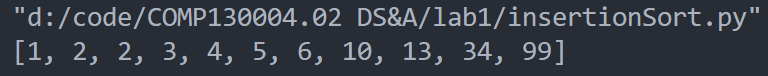
\includegraphics[width=0.8\textwidth]{insertionSort.png}
    \caption{Output of insertionSort}
\end{figure}


\section{}
Write code for merge sort.\\

\textbf{Solution}: See mergeSort.py.
\begin{lstlisting}
def merge(left, right): # merge two sorted arrays
    result = []
    i = 0
    j = 0
    leftlen = len(left)
    rightlen = len(right)
    while i < leftlen and j < rightlen:
        if left[i] < right[j]:
            result.append(left[i]) # append the smaller value
            i += 1
        else:
            result.append(right[j])
            j +=1
    result += left[i:] # append the rest of the values
    result += right[j:] # append the rest of the values
    return result

def mergeSort(array):
    n = len(array)
    if n == 1:
        return array
    else:
        mid = int(n/2) # split the array in half
        left = array[:mid] # left half
        right = array[mid:] # right half
        left = mergeSort(left) # recursively sort the left half
        right = mergeSort(right) # recursively sort the right half
        return merge(left, right) # merge the two sorted halves
\end{lstlisting}
\textbf{Code interpretation:} \\
The code defines a function $\it{mergeSort}$ which takes an array as input and returns the sorted array. 
If the length of the array is $1$, it returns the array. Otherwise, it splits the array in half and recursively calls $\it{mergeSort}$ on the two halves. 
Then it calls $\it{merge}$ to merge the two sorted halves. The merge function compares the first element of the two arrays and appends the smaller one to the result array, and then it increments the index of the array from which the smaller value is appended.
After one of the arrays is empty, it appends the rest of the values in the other array to the result array. \\
\textbf{Result analysis:} \\
The code is tested with the following array: $[5, 2, 4, 6, 1, 3, 99, 10, 34, 2, 13]$. As shown in Figure 2, the code returns the sorted array $[1, 2, 2, 3, 4, 5, 6, 10, 13, 34, 99]$ successfully.
\begin{figure}[H]
    \centering
    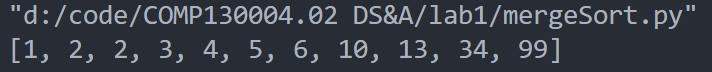
\includegraphics[width=0.8\textwidth]{mergeSort.png}
    \caption{Output of mergeSort}
\end{figure}


\section{}
The running time of merge sort can be improved in practice by taking advantage of the fast 
running time of insertion sort when its input is "nearly" sorted. When merge sort is called on a 
subarray with fewer than $k$ elements, use insertion sort to sort the subarray. Argue that this sorting 
algorithm runs in $O(f(n, k))$ expected time. What is $f(n, k)$ and how should k be picked, both in 
theory and in practice by experiments?\\

\textbf{Solution}:\\
The recursion stops when the length of the array is less than $k$. If $h$ is the depth of the recursive tree, we have $\frac{n}{2^h} = k$, which gives $h = \log \frac{n}{k}$. 
The running time of each level is $O(n)$, so the total merge time is $O(n \log \frac{n}{k})$. 
Running insertion sort on the $\frac{n}{k}$ subarrays of length $k$ takes $O(k^2)$ time each on average. So the total running time is $O(nk + n \log \frac{n}{k})$, and $f(n,k) = nk + n \log \frac{n}{k}$.\\

In theory, $k$ should be picked such that $f(n,k)$ is minimized. We have $\frac{\partial f(n,k)}{\partial k} = n - \frac{n}{k} = 0$, this gives $k = 1$, which is not a satisfactory value.
We have to consider the constant factors, as big-$O$ notation ignores them but they actually affects the running time. If the running time is $c_1 n \log \frac{n}{k} + c_2 nk$, then $\frac{\partial f(n,k)}{\partial k} = - c_1 \frac{n}{k} + c_2 n = 0$, which gives $k = \frac{c_1}{c_2}$.
Note that the constants are dependent of the machine, and some lower order terms are ignored, so theoretically we cannot find the optimal value of $k$ directly.\\

In practice, we can pick $k$ by running experiments. We can run the algorithm with different values of $k$ and pick the one that gives the smallest running time. 
The code below is used to find the best $k$ according to various size $n$. For every $n= 10000, 10500, \ldots, 20000$, we run the combine sort with $k$ ranging from $10$ to $50$ with step size $2$.
To prevent the randomness of the input array from affecting the result, we run the algorithm $10$ times for each $k$ and take the average running time.\\
\begin{lstlisting}
import time
import matplotlib.pyplot as plt
import random
from collections import Counter

def insertionSort(array):
    n = len(array)
    for j in range(1,n):
        key = array[j]
        i = j - 1
        while i >= 0 and key < array[i]:
            array[i+1] = array[i]
            i = i - 1
        array[i+1] = key
    return array

def merge(left, right):
    i = j = 0
    result = []
    while i < len(left) and j < len(right):
        if left[i] <= right[j]:
            result.append(left[i]) 
            i += 1
        else:
            result.append(right[j])
            j += 1
    result += left[i:]
    result += right[j:]
    return result

def combineSort(array, k):
    n = len(array)
    if n <= k: # if array size is less than k, use insertion sort
        return insertionSort(array)
    else: # else, split array in half and recursively call combineSort
        mid = n//2
        left = array[:mid]
        right = array[mid:]
        left = combineSort(left, k)
        right = combineSort(right, k)
        return merge(left, right)

def fine_best_k(arrsize, krange):
    random.seed(203) # set seed to 203
    array = [random.randint(0, 1000000) for _ in range(arrsize)] # generate random array
    best_k = 0
    best_time = 9999999999 # set best time to a rather large number

    for k in krange: # max subarray size for insertion sort
        total_time = 0
        avg_time = 0
        for i in range(1,10): # run 10 times and take average
            start = time.time()
            combineSort(array, k) # call combine sort
            end = time.time()
            total_time += end - start
        avg_time = total_time/10
        
        if avg_time < best_time:
            best_time = avg_time
            best_k = k
    return best_k


sizerange = range(10000, 20000, 500) # array size range
k_record = [] # record best k for each array size
krange = range(10, 51, 2) # max subarray size for insertion sort. The best k mostly lies in 10~50
for arraysize in sizerange:
    k_record.append(fine_best_k(arraysize, krange))
    
count = Counter(k_record)
print(count.most_common(1)[0][0]) # print k with the most frequency
plt.plot(sizerange, k_record, 'b--') # plot array size vs best k
plt.show()
\end{lstlisting}
The plot of array size vs best $k$ is shown in Figure 3. From the figure, we notice that $k$ is not a constant, but 
in this experiment $k = 20$ is the best value for most array sizes, for it has the highest frequency.\\
\begin{figure}[H]
    \centering
    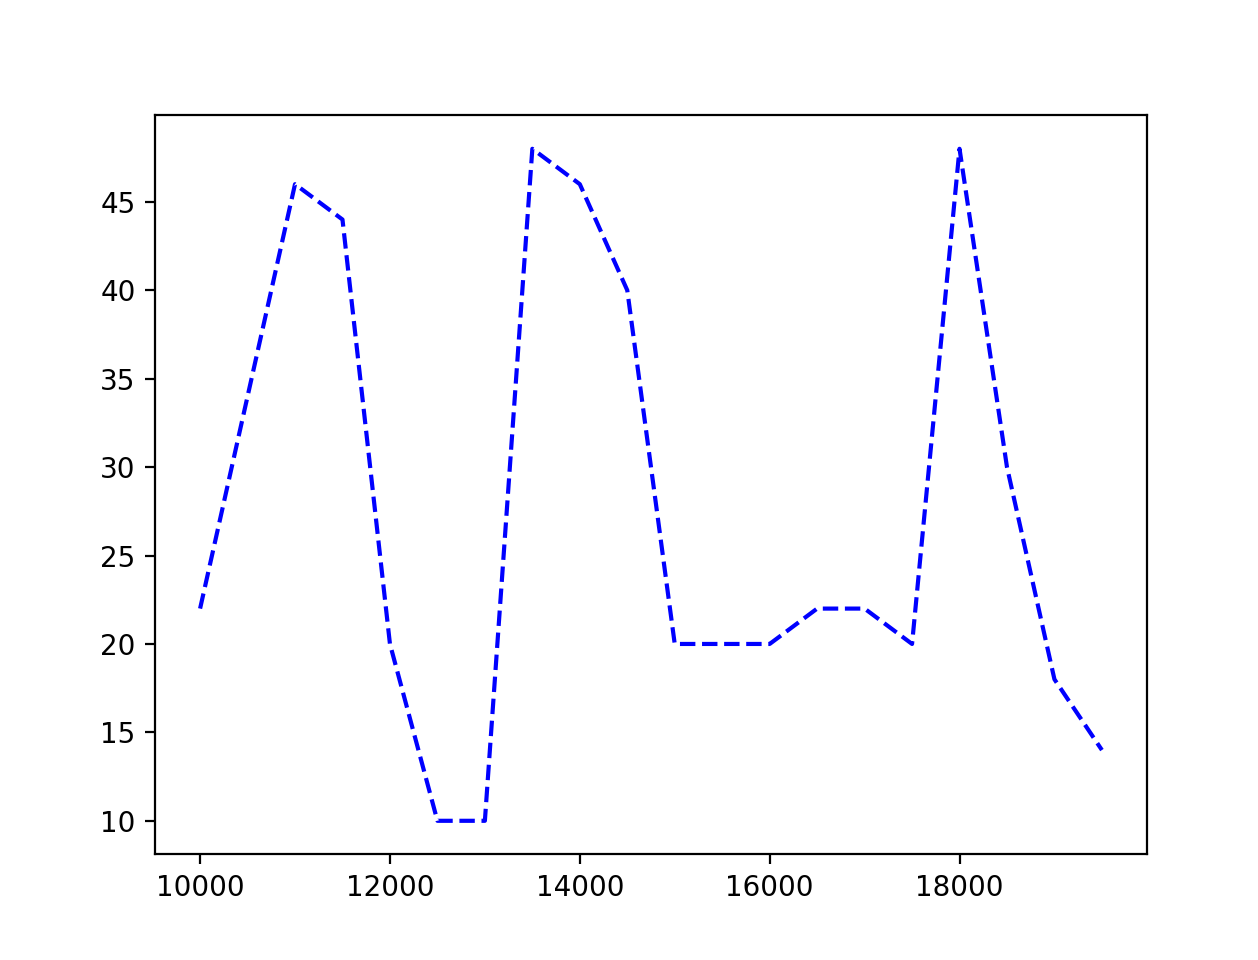
\includegraphics[width=0.8\textwidth]{best k.png}
    \caption{array size vs best k}
\end{figure}
There are many reasons why the best $k$ is not a constant. For example, the constants in the running time of insertion sort and merge sort are dependent of the machine, so they can vary a little.
Additionally, the cache of the computer can affect the running time of insertion sort, which is not considered in the theoretical analysis. But we can still conclude that $k$ can be taken as a constant in practice, for the best $k$ is not changing dramatically with the array size.\\
    
\section{}
Write code for improved version of sorting algorithm which combines merge sort with insertion sort.\\

\textbf{Solution}: See combine\_insert\_merge.py.
\begin{lstlisting}
k = 20

def insertionSort(array):
    n = len(array)
    for j in range(1,n):
        key = array[j]
        i = j - 1
        while i >= 0 and key < array[i]:
            array[i+1] = array[i]
            i = i - 1
        array[i+1] = key
    return array

def merge(left, right):
    i = j = 0
    result = []
    while i < len(left) and j < len(right):
        if left[i] <= right[j]:
            result.append(left[i]) 
            i += 1
        else:
            result.append(right[j])
            j += 1
    result += left[i:]
    result += right[j:]
    return result
    
def combineSort(array, k):
    n = len(array)
    if n <= k: # if array size is less than k, use insertion sort
        return insertionSort(array)
    else: # else, split array in half and recursively call combineSort
        mid = n//2
        left = array[:mid]
        right = array[mid:]
        left = combineSort(left, k)
        right = combineSort(right, k)
        return merge(left, right)
\end{lstlisting}
\textbf{Code interpretation:} \\
The code defines a function $\it{combineSort}$ which takes an array as input and returns the sorted array. It combines insertion sort and merge sort with a threshold $k = 20$ for calling $\it{insertionSort}$, according to
the experiment result above.\\
\textbf{Result analysis:} \\
The code is tested with a randomly generated array with size $50$. As shown in Figure 4, the code returns the sorted array successfully.
\begin{figure}[H]
    \centering
    \includegraphics[width=0.8\textwidth]{combineSort.png}
    \caption{Output of combineSort}
\end{figure}

\end{document}